%!TEX root = paper.tex
\subsection{Solitary wave on a composite beach} \label{sec:B_compositebeach}
This is an laboratory experiment conducted at the Coastal Engineering Laboratory of the U.S. Army Corps of Engineers and it is described in \url{http://nctr.pmel.noaa.gov/benchmark/Solitary_wave/}, \url{http://chl.erdc.usace.army.mil/chl.aspx?p=s&a=Projects;36}. 
A linear solitary (better called single) wave is propagating over a stepwise increasing bathymetry and it is reflected at a vertical wall on the right boundary. Different wave gauges measure the surface elevation and the runup on the vertical wall. 
The experimental data serve for validation of the models. Additionally to the experimental data, a linear analytic solution is provided, s.t. verification of our models is also tested.

Three different cases A, B, C with different target wave heights $a_t$, actual (measured) wave heights $a$ and distances $L$ of gauge $G4$ to the first step in the bathymetry at gauge $G5$. Table \ref{tab:compositebeach_cases} displays the three different cases and belonging data. We only consider case A at the moment. Measured runup data can be found in table \ref{tab:compositebeach_runup}, but are not compared yet to the simulations.

\begin{table}[htbp]
\begin{tabular}{lllll}
\textbf{Case} & \textbf{target $a_t / d$} & \textbf{actual $a / d$} & \textbf{dist. G4 to G5 [m]} & \textbf{dist. G4 to Wall [m]}  \\
\toprule
A       &     0.05   & 0.039    &   2.4   &  10.59     \\
B       &     0.30   & 0.264    &   0.89  &   9.17     \\
C       &     0.70   & 0.696    &    0.64  &   8.83    \\
\bottomrule
\end{tabular}
\caption{Data of three different cases}
\label{tab:compositebeach_cases}
\end{table}


\begin{table}[htbp]
\begin{tabular}{lll}
\textbf{Case} & \textbf{Runup R [cm]} & \textbf{R / d} \\
\toprule
A       &        2.74  &  0.13 \\
B       &       45.72  &  2.10 \\
C       &       27.43  &  1.26 \\
\bottomrule
\end{tabular}
\caption{Runup laboratory results of three different cases}
\label{tab:compositebeach_runup}
\end{table}


The initial condition is prescribed as 
\begin{itemize}
 \item a linear analytic solitary wave solution
\begin{align}
\xi(\bx,t)&=a_t \ \text{cosh}^{-2}(K(x-ct-x_0)), \\
u(\bx,t)&=c\frac{\xi(\bx,t)}{d},
\end{align}
with the initial target amplitude $a_t$, propagation velocity $c=\csw$ on a stepwise reduced depth starting from $d=0.218 \, \text{m}$ with scale factor $K=\sqrt{\left(\frac{3a_t}{4d^3}\right)}$ and displacement $x_0=10.59$, s.t. the initial solitary wave has its maximum at gauge G4 while the entire domain length is $L=24 \, \text{m}$. The simulation time is $20$ seconds. 
 \item the first option in \url{https://github.com/rjleveque/nthmp-benchmark-problems/blob/master/BP05-ElenaT-Solitary_wave_on_composite_beach_laboratory/BP5_description.pdf}. The velocities are set to zero and the doubled initial surface elevation $2\xi$ is prescribed at $x=0$. A doubled domain length of $L=48 \, \text{m}$ ensures that the waves reflected at the left boundary are not disturbing the solution. The simulation time is $40$ seconds.
\end{itemize}
We impose reflecting boundary conditions at the boundary in x-direction and periodic boundary conditions in y-direction. For the setup see figure \ref{fig:compositebeach_setup}. 
Because the analytic solution belongs to the linear SWE, corresponding models are expected to represent very good coincidence with this analytic solution.

\begin{figure}[htbp]
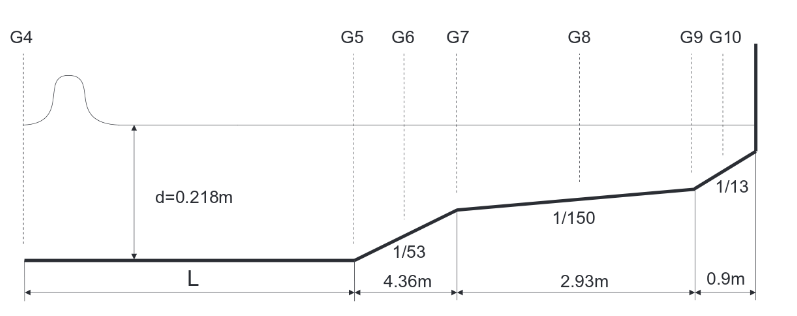
\includegraphics[width=\textwidth]{compositebeach_setup}
\caption{Setup of the testcase solitary wave on a composite beach}
\label{fig:compositebeach_setup}
\end{figure}

\subsubsection{Results of \nh\ model}
The results of the first and the seconds option are shifted by 271.5s to match the initial wave at gauge G4. Both are also scaled with a factor of $\frac{0.037}{0.05}$. % because $0.037$m seems to be the actual amplitude instead of $0.039$.
No difference between both options is visible in the figures then. Hence, we only plot the results of the (cheaper) first option using the linear SWE model and also the following results obtained with the \nh\ model.

Figures \eqref{fig:nh_compositebeach_ana_nh_Lhy} and \eqref{fig:nh_compositebeach_lab_nh_Lhy} display the comparison of the linear SWE with the linear analytic solution and experimental data, respectively.
The models results compared to the analytic solution are very good, while at gauges G9 and G10 a mismatch is visible, because the nonlinear regime is entered here (d $\in [0.047,0.117]$m, $a\approx0.008$m), for which the linear model is not suited.
The comparison to the experimental data reveals less dispersion and reduced amplitudes, although the overall match is also satisfactory.

Figures \eqref{fig:nh_compositebeach_ana_nh_Nnh12} and \eqref{fig:nh_compositebeach_lab_nh_Nnh12} display the comparison of the \nh\ equations using both the linear and the quadratic pressure profile with the linear analytic solution and experimental data, respectively. The \nh\ wave profile represents well the amplitudes, the shape of the propagating wave, the propagation velocities and also the developed dispersive wave train after reflecting of the laboratory surface elevation. The agreement with the linear analytic solution is worse, but still okay.
When wave hits step, the numerical sea surface height is not as much increased as the amplitude of exp data. 

Differences between both vertical pressure profiles are small, because dispersive effects become more significant after longer simulation time. However, the tendency of the linear profile to overestimate amplitudes, which was also visible in figure \ref{fig:nh_solitarywave}, is confirmed here, too. Additionally, we see that is also true not only for global maxima, but also for local maxima.

The analytic solution is a good test for the verification of the linear SWE model, whereas the laboratory data show its limits of applicability as well as that the dispersive model gives a more accurate physical representation of the experimental data.

Need to do: wq refl b.c. may be not good enough (not explicit treatment at the moment), edge integrals are missing.


\begin{figure}[htbp]
\begin{minipage}{\textwidth}
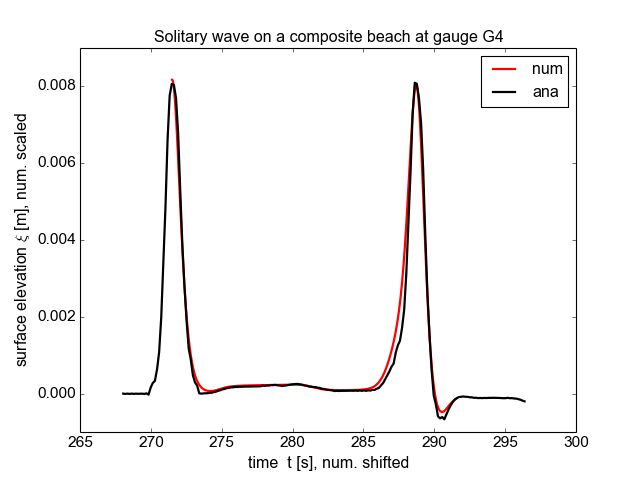
\includegraphics[width=0.48\textwidth]{compositebeach_ana_G4_nh_Lhy}
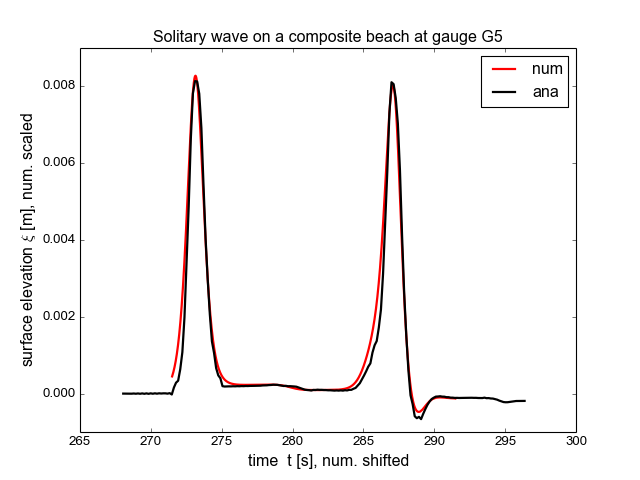
\includegraphics[width=0.48\textwidth]{compositebeach_ana_G5_nh_Lhy}
\end{minipage} \\
\begin{minipage}{\textwidth}
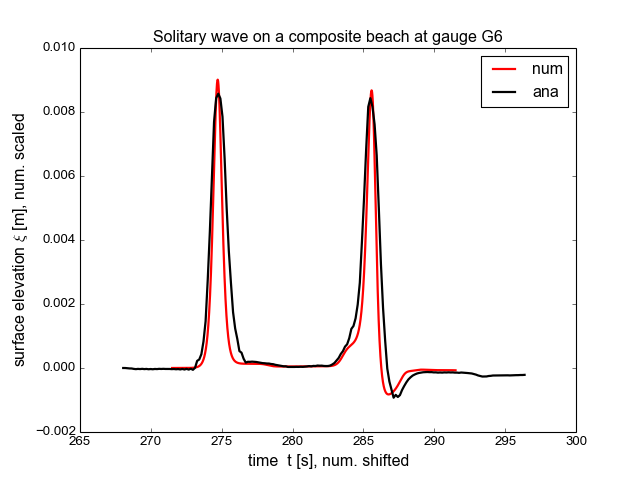
\includegraphics[width=0.48\textwidth]{compositebeach_ana_G6_nh_Lhy}
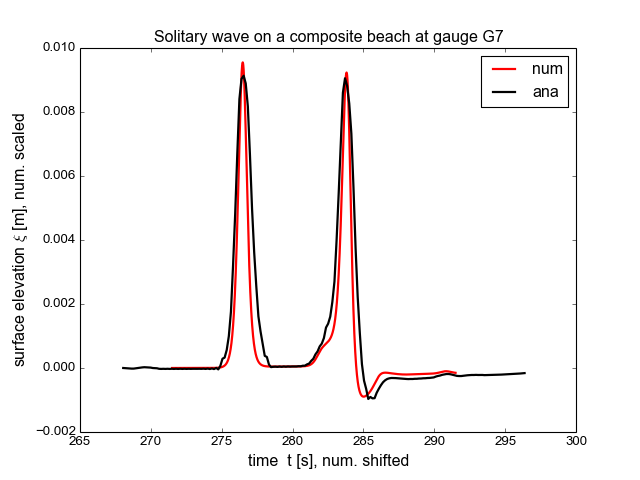
\includegraphics[width=0.48\textwidth]{compositebeach_ana_G7_nh_Lhy}
\end{minipage} \\
\begin{minipage}{\textwidth}
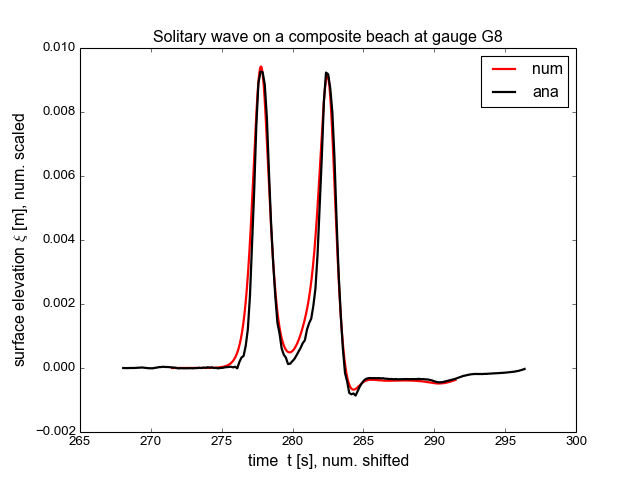
\includegraphics[width=0.48\textwidth]{compositebeach_ana_G8_nh_Lhy}
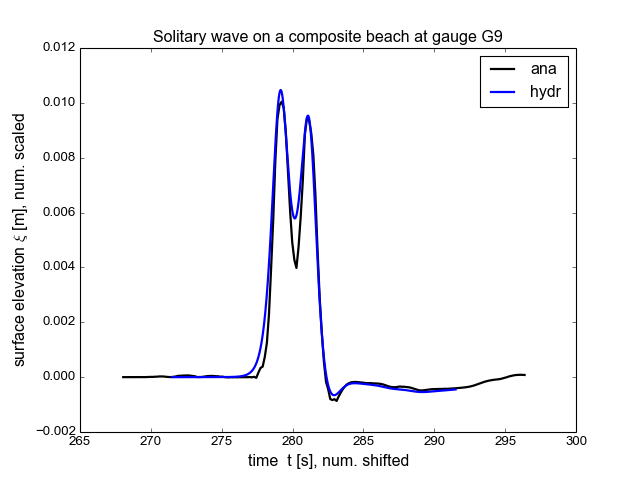
\includegraphics[width=0.48\textwidth]{compositebeach_ana_G9_nh_Lhy}
\end{minipage} \\
\begin{minipage}{\textwidth}
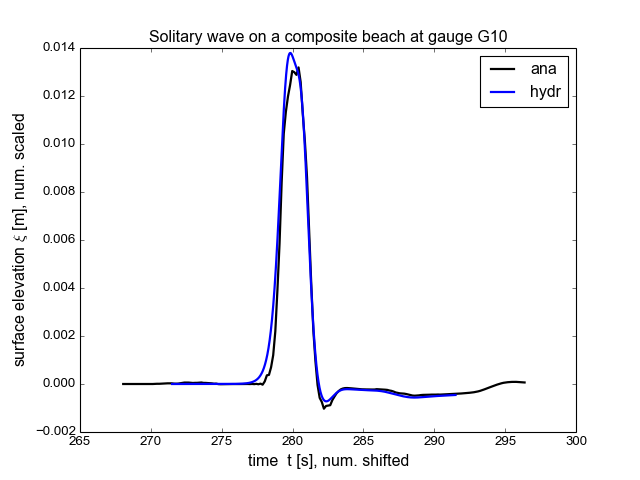
\includegraphics[width=0.48\textwidth]{compositebeach_ana_G10_nh_Lhy}
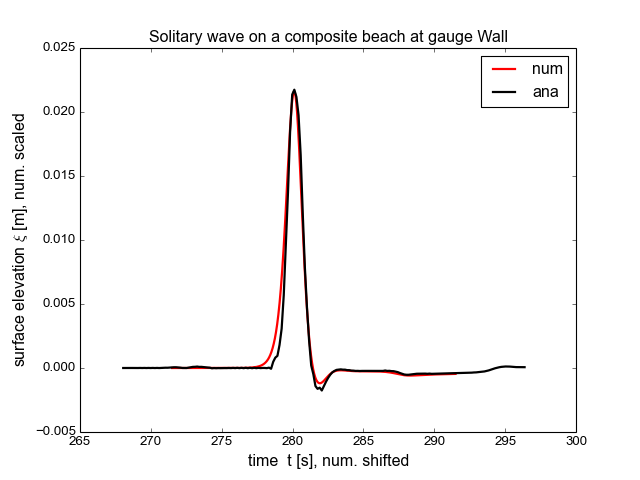
\includegraphics[width=0.48\textwidth]{compositebeach_ana_Wall_nh_Lhy}
\end{minipage}
\caption{Comparison of the analytical (black) sea surface height of the
solitary wave with the simulation results of the \nh\ model in its version of linear shallow water equations (blue)}
\label{fig:nh_compositebeach_ana_nh_Lhy}
\end{figure}

\begin{figure}[htbp]
\begin{minipage}{\textwidth}
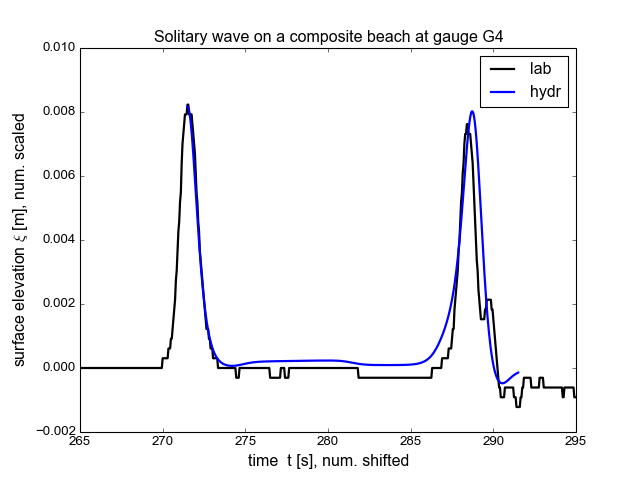
\includegraphics[width=0.48\textwidth]{compositebeach_lab_G4_nh_Lhy}
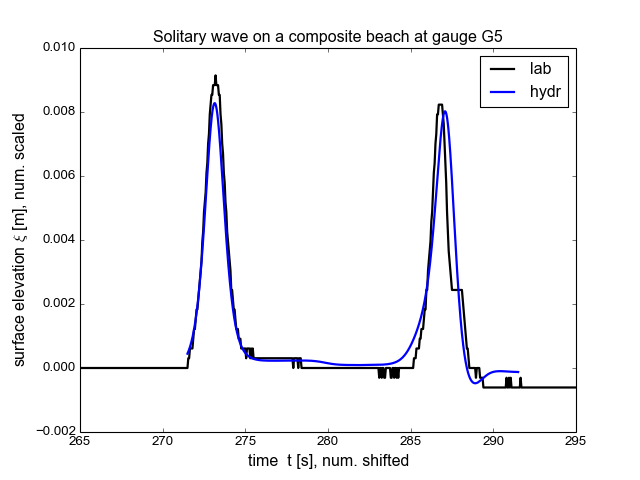
\includegraphics[width=0.48\textwidth]{compositebeach_lab_G5_nh_Lhy}
\end{minipage} \\
\begin{minipage}{\textwidth}
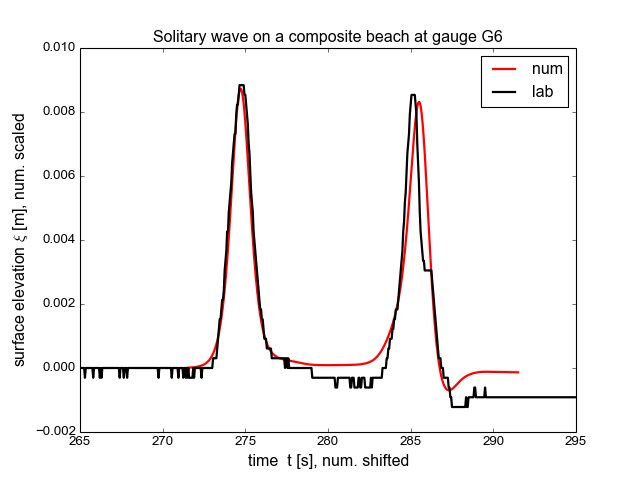
\includegraphics[width=0.48\textwidth]{compositebeach_lab_G6_nh_Lhy}
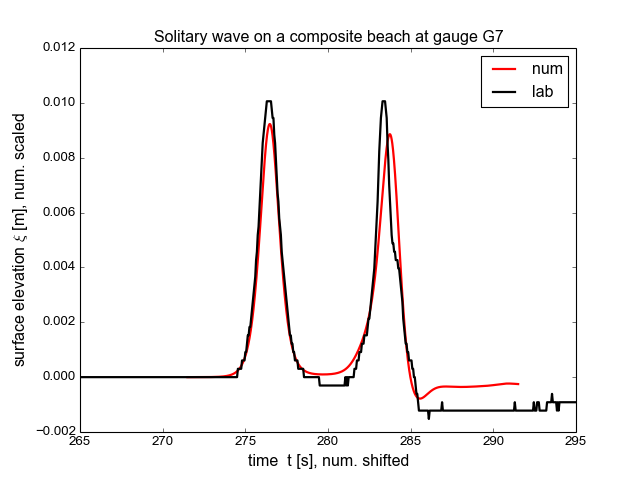
\includegraphics[width=0.48\textwidth]{compositebeach_lab_G7_nh_Lhy}
\end{minipage} \\
\begin{minipage}{\textwidth}
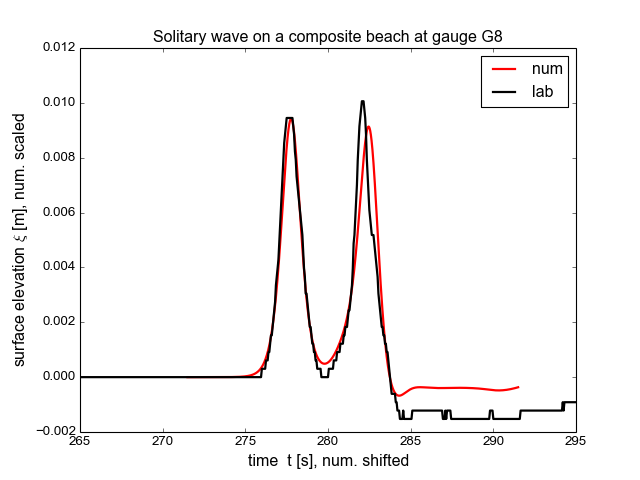
\includegraphics[width=0.48\textwidth]{compositebeach_lab_G8_nh_Lhy}
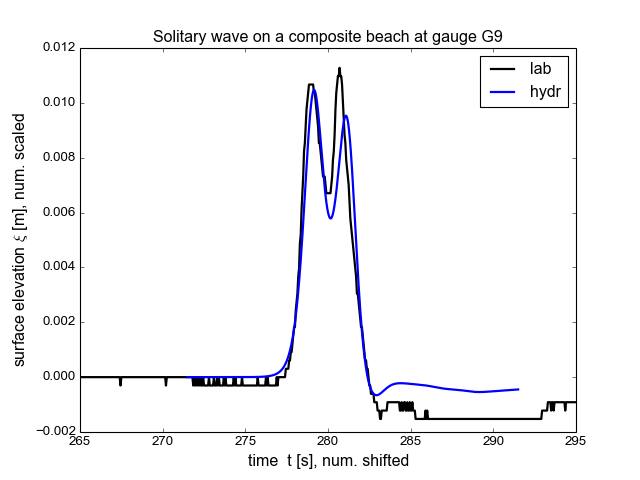
\includegraphics[width=0.48\textwidth]{compositebeach_lab_G9_nh_Lhy}
\end{minipage} \\
\begin{minipage}{0.48\textwidth}
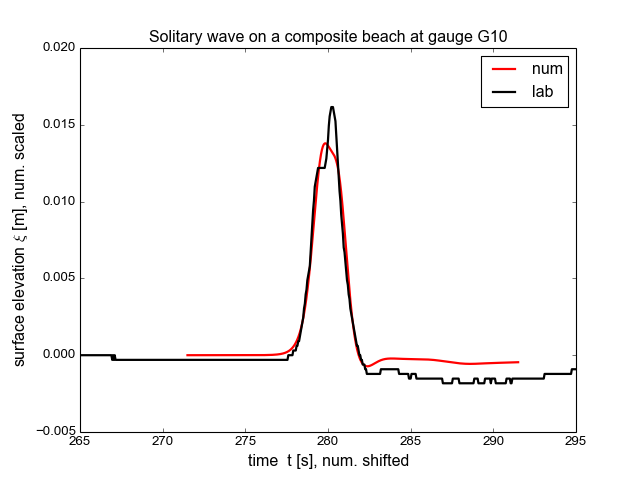
\includegraphics[width=\textwidth]{compositebeach_lab_G10_nh_Lhy}
\end{minipage} 
\begin{minipage}{0.45\textwidth}
\begin{tabular}{lll}
\textbf{Data} & \textbf{Runup} & \textbf{R / d} \\
              & \textbf{R [cm]} &  \\
\toprule
Exp.  &  2.74   &  0.13 \\
Model hydr. &  2.13   &  0.0978 \\
\end{tabular}
\end{minipage}
\caption{Comparison of the experimental (black) sea surface height of the
solitary wave with the simulation results of the \nh\ model in its version of linear shallow water equations (blue). The model runup is also scaled with 0.75.}
\label{fig:nh_compositebeach_lab_nh_Lhy}
\end{figure}



\begin{figure}[htbp]
\begin{minipage}{\textwidth}
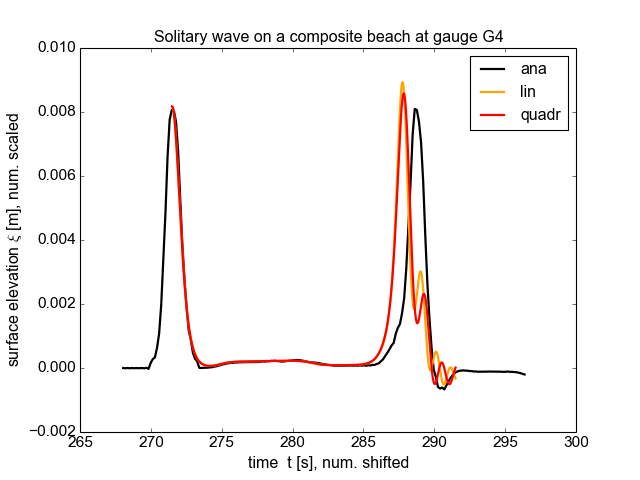
\includegraphics[width=0.48\textwidth]{compositebeach_ana_G4_nh_Nnh12}
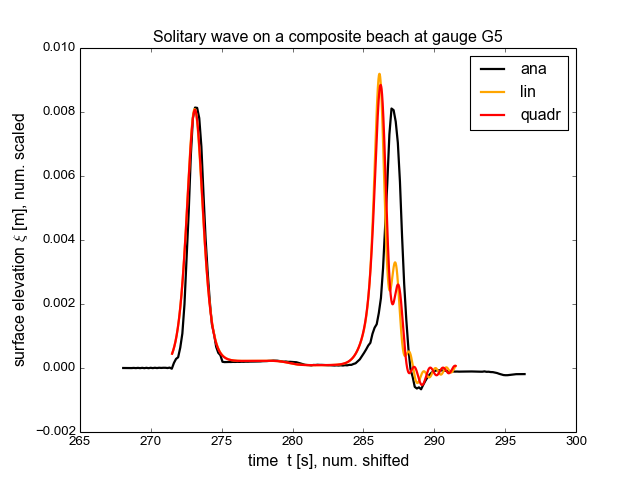
\includegraphics[width=0.48\textwidth]{compositebeach_ana_G5_nh_Nnh12}
\end{minipage} \\
\begin{minipage}{\textwidth}
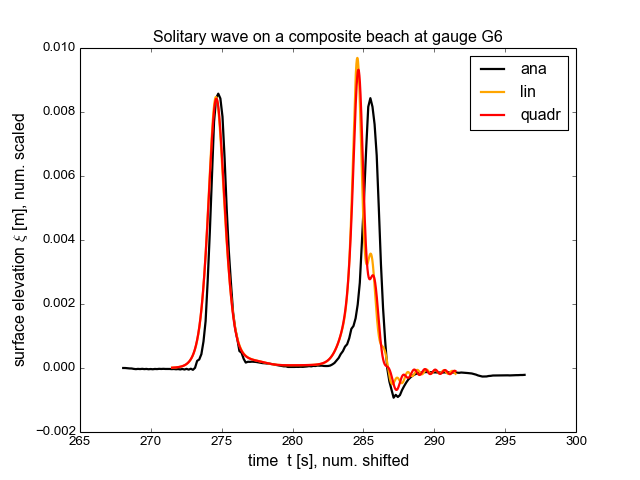
\includegraphics[width=0.48\textwidth]{compositebeach_ana_G6_nh_Nnh12}
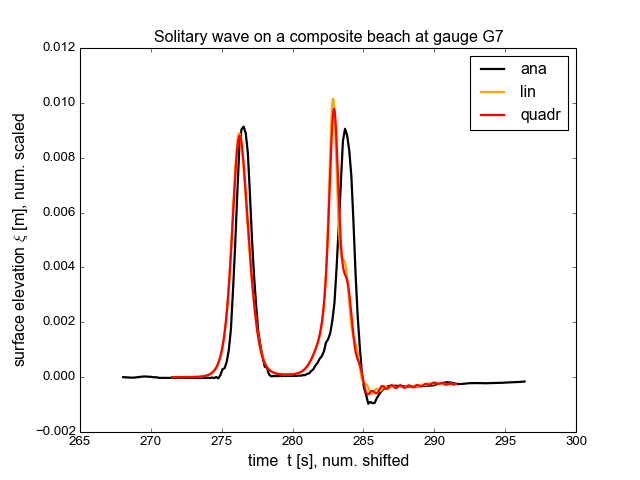
\includegraphics[width=0.48\textwidth]{compositebeach_ana_G7_nh_Nnh12}
\end{minipage} \\
\begin{minipage}{\textwidth}
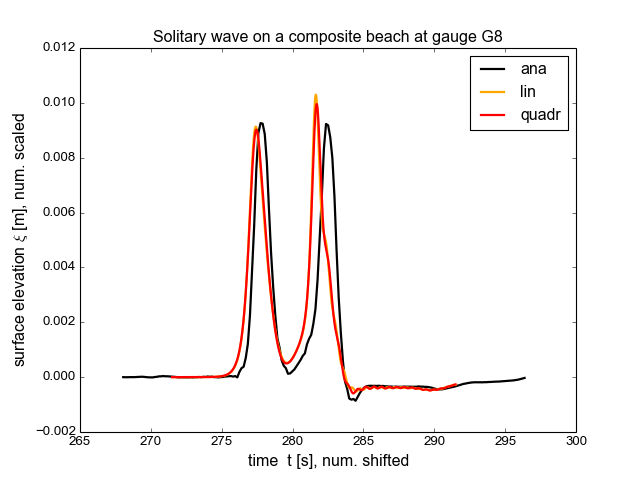
\includegraphics[width=0.48\textwidth]{compositebeach_ana_G8_nh_Nnh12}
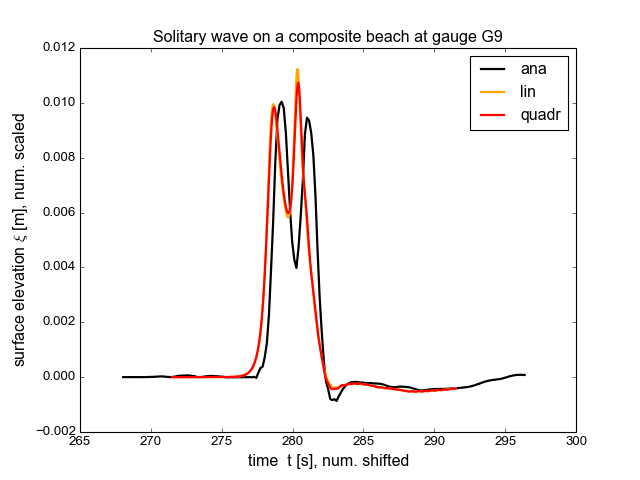
\includegraphics[width=0.48\textwidth]{compositebeach_ana_G9_nh_Nnh12}
\end{minipage} \\
\begin{minipage}{\textwidth}
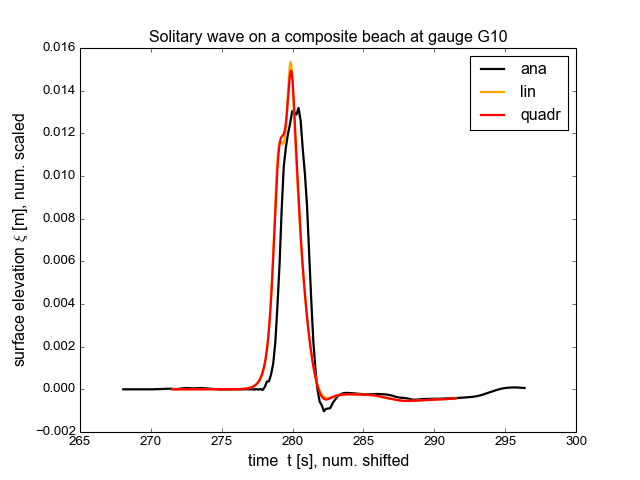
\includegraphics[width=0.48\textwidth]{compositebeach_ana_G10_nh_Nnh12}
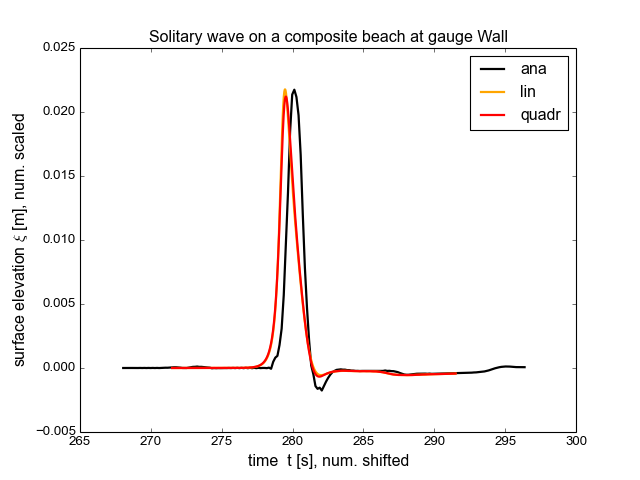
\includegraphics[width=0.48\textwidth]{compositebeach_ana_Wall_nh_Nnh12}
\end{minipage}
\caption{Comparison of the analytical (black) sea surface height of the
solitary wave with the simulation results of the \nh\ model in its \nh\ version using the linear (yellow) and the quadratic vertical pressure profile (red)}
\label{fig:nh_compositebeach_ana_nh_Nnh12}
\end{figure}

\begin{figure}[htbp]
\begin{minipage}{\textwidth}
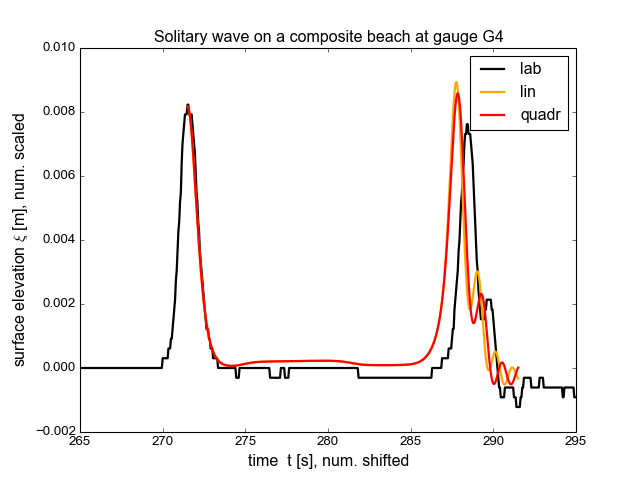
\includegraphics[width=0.48\textwidth]{compositebeach_lab_G4_nh_Nnh12}
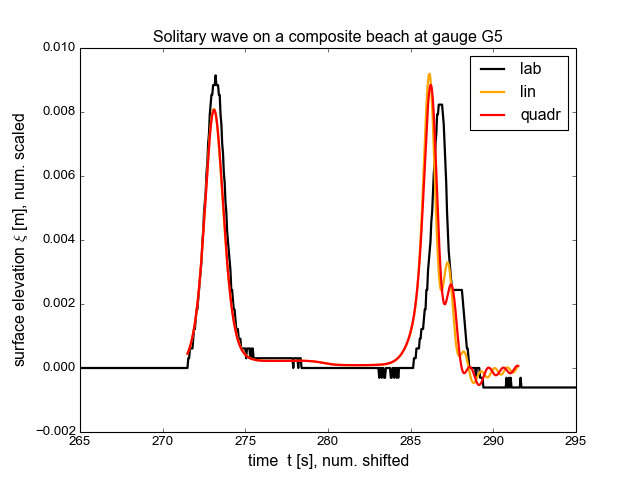
\includegraphics[width=0.48\textwidth]{compositebeach_lab_G5_nh_Nnh12}
\end{minipage} \\
\begin{minipage}{\textwidth}
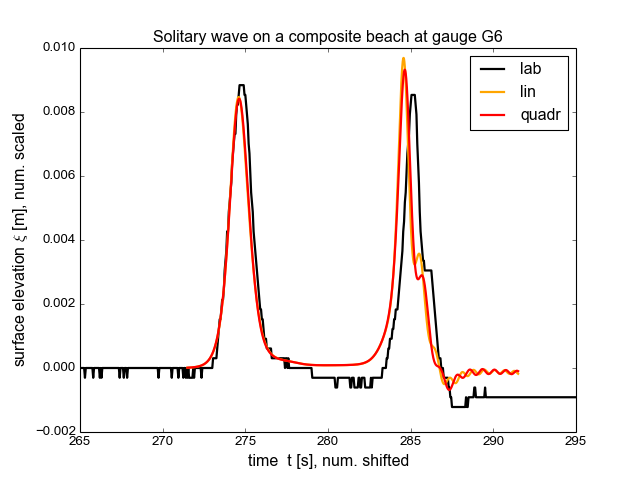
\includegraphics[width=0.48\textwidth]{compositebeach_lab_G6_nh_Nnh12}
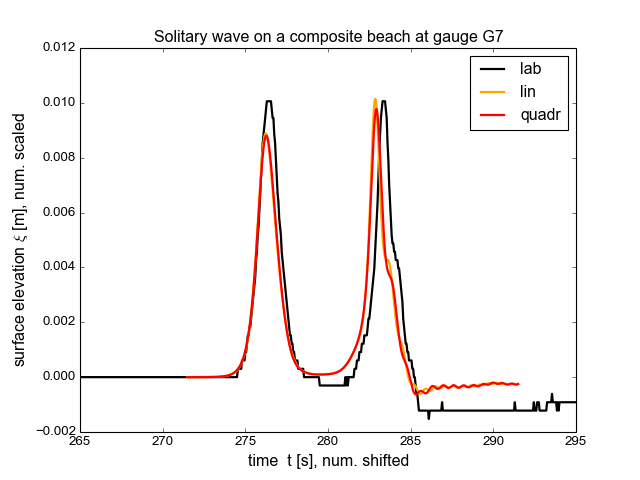
\includegraphics[width=0.48\textwidth]{compositebeach_lab_G7_nh_Nnh12}
\end{minipage} \\
\begin{minipage}{\textwidth}
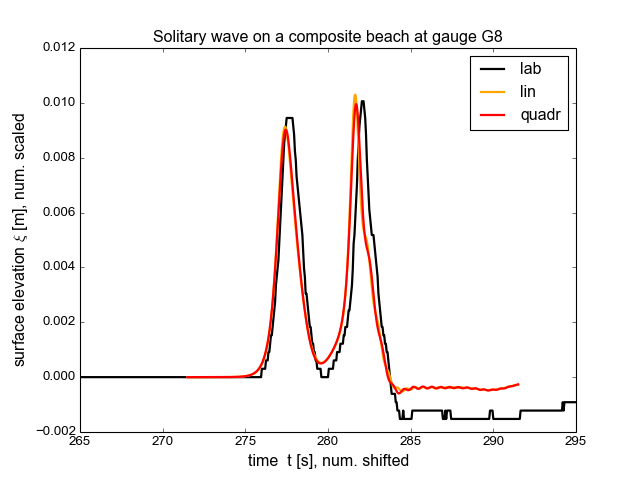
\includegraphics[width=0.48\textwidth]{compositebeach_lab_G8_nh_Nnh12}
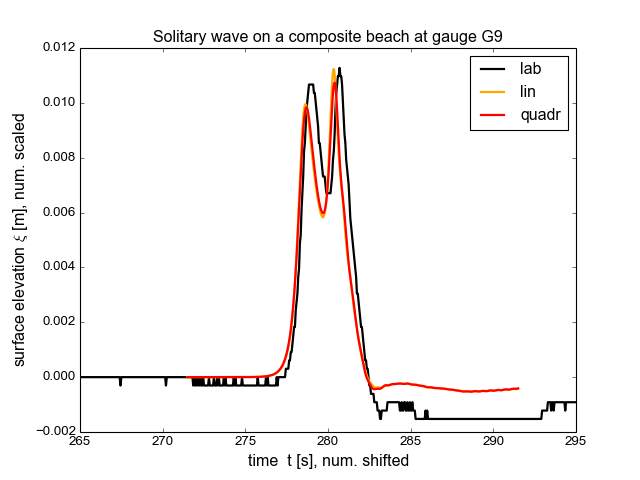
\includegraphics[width=0.48\textwidth]{compositebeach_lab_G9_nh_Nnh12}
\end{minipage} \\
\begin{minipage}{0.48\textwidth}
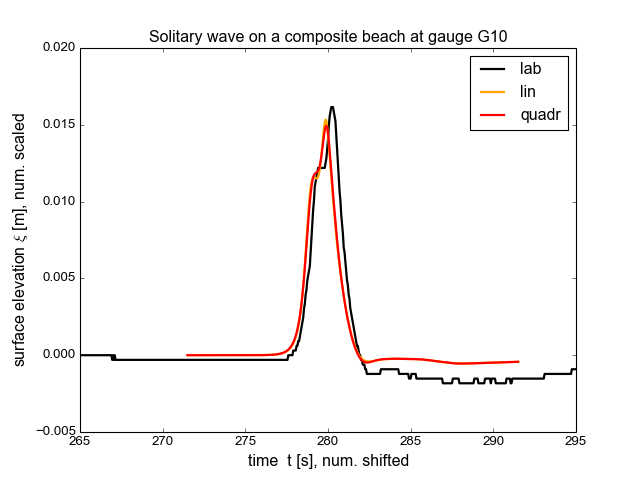
\includegraphics[width=\textwidth]{compositebeach_lab_G10_nh_Nnh12}
\end{minipage} 
\begin{minipage}{0.45\textwidth}
\begin{tabular}{lll}
\textbf{Data} & \textbf{Runup} & \textbf{R / d} \\
              & \textbf{R [cm]} &  \\
\toprule
Exp.  &  2.74   &  0.13 \\
Model lin.&  2.18   &  0.10 \\
Model quadr.&  2.12   &  0.097 \\
\end{tabular}
\end{minipage}
\caption{Comparison of the experimental (black) sea surface height of the
solitary wave with the simulation results of the \nh\ model in its \nh\ version using the linear (yellow) and the quadratic vertical pressure profile (red). The model runup is also scaled with 0.75.}
\label{fig:nh_compositebeach_lab_nh_Nnh12}
\end{figure}
